\documentclass[journal=jctcce,manuscript=article,maxauthors=999]{achemso}

\usepackage{amsmath,amssymb,mathtools}
\usepackage{booktabs}
\usepackage{siunitx}
\usepackage{orcidlink}
\usepackage{verbatim}
\usepackage{tikz}
\usetikzlibrary{arrows.meta,backgrounds,fit,positioning}
\definecolor{MerlinoBlue}{HTML}{245C73}
\definecolor{MerlinoTeal}{HTML}{2F8F83}
\definecolor{MerlinoGold}{HTML}{C88A2D}
\definecolor{MerlinoSlate}{HTML}{4A5561}
\definecolor{MerlinoInk}{HTML}{263238}
\emergencystretch=2em

\title{Non-Redundant and Symmetry-Adapted Coordinates for Black-Box Molecular Structure Refinement}

\author{Vincenzo Barone\,\orcidlink{0000-0001-6420-4107}}
\affiliation{INSTM, National Interuniversity Consortium for Materials Science and Technology, via G. Giusti 9, 50121 Firenze, Italy}
\email{vincebarone52@gmail.com}

\keywords{semiexperimental equilibrium structures, rotational spectroscopy, generalized internal coordinates, least squares, Kraitchman equations}

\begin{document}

\begin{abstract}

Semiexperimental equilibrium structures combine high-resolution rotational
spectroscopy with computed vibrational and electronic corrections. The
least-squares refinement depends on the coordinate model used to connect
observables, constraints, and structural parameters. Z-matrices are compact for
simple acyclic molecules; in rings, fused systems, and bridged frameworks they
introduce reference-tree choices, derived ring quantities, and manually selected
symmetry relationships.

We present \texttt{SEfit}, a black-box structure-refinement framework in which
the input structure is Cartesian and the active coordinate model is generated
from molecular topology and symmetry. Two representations are available. The
first is a non-redundant symmetry-adapted generalized-internal-coordinate basis
built from homogeneous primitive blocks of stretches, bends, torsions,
out-of-plane motions, and ring coordinates. The second is a symmetry-adapted
Cartesian displacement basis obtained after exact removal of translations and
rotations. In both representations all atoms enter through the same Cartesian
topology, and only the totally symmetric active subspace is refined.

The chemical interface remains internal-coordinate based. Constraints,
predicates, and parameter classes are specified as primitive relations because
bond lengths, valence angles, dihedrals, and local hydrogen frames are the
quantities that carry chemical meaning. These relations are projected onto
either active basis through the Wilson matrix or the corresponding
primitive-coordinate derivative projector, preserving chemically defined
constraints and rigorous uncertainty propagation.

\texttt{SEfit} integrates moment-of-inertia fitting, vibrational and electronic
corrections, predicate observations, parameter classes, reduced-dimensionality
hydrogen models, statistical diagnostics, and human-readable reports within a
single Cartesian/topology-based refinement workflow.

Glycolaldehyde is used as a standard acyclic reference. Glycine I and II test
constrained refinements with, respectively, a C$_s$ symmetry model and a
fully non-symmetric functional-constraint model, whereas cyclopentadiene,
nitrobenzene, azulene, and norcamphor probe cyclic, planar aromatic,
polycyclic, and bridged cases. Across these benchmarks the
generalized-internal-coordinate and symmetry-Cartesian refinements give the
same numerical ranks, effective dimensionalities, and rotational residuals,
while final structural parameters and uncertainties remain chemically
interpretable.

\end{abstract}


\section{Introduction}

Accurate equilibrium molecular structures are central to rotational
spectroscopy, thermochemistry, force-field development, and the validation of
electronic-structure methods.\cite{Demaison2011EquilibriumStructures,PuzzariniStanton2023}
More generally, structure determination from experimental observables is a
coordinate-dependent inverse problem. The data constrain a Cartesian geometry,
but the fitted variables determine conditioning, constraints, correlations, and
propagated uncertainties. Rotational spectroscopy is a stringent example because
rotational constants probe the molecular mass distribution with high precision,
whereas semiexperimental ($r_e^{\mathrm{SE}}$) structures require vibrational
and sometimes electronic corrections to convert ground-state constants into
equilibrium information.\cite{Costain1958,Pawlowski2002,Piccardo2015B3LYP,Penocchio2015B2PLYP}

Modern semiexperimental and rotational-structure fitting programs and
workflows, including the \texttt{MSR} molecular-structure-refinement program
and the \texttt{STRFIT} structure-fitting program distributed with
\texttt{PROSPE},\cite{Mendolicchio2017MSR,KisielPROSPE,Kanzow2025PCCP} have
established robust statistical principles: fit moments of inertia or otherwise
well-conditioned observables, include theoretical predicates when experimental
information is incomplete, and propagate the covariance matrix to derived
structural parameters.\cite{Bartell1975Predicate} The remaining bottleneck is
the coordinate model rather than the least-squares formalism.
This issue is easily hidden in small acyclic molecules, where a single
Z-matrix reference tree can represent the important distances and angles
without serious ambiguity.

Recent automated workflows have substantially extended the practical reach of
semiexperimental refinement by coupling computed starting geometries, efficient
second-order vibrational perturbation theory (VPT2)-based vibrational
corrections, and reduced-dimensionality refinements in a largely black-box
pipeline.\cite{Mendolicchio2025FastDvib} \texttt{SEfit} uses such computed
geometries and correction data as upstream inputs and replaces the remaining
user-defined Z-matrix layer with a topology-driven coordinate engine.

The same construction is not unique for rings, fused systems, and bridged
frameworks. A Z-matrix is a tree representation of a molecular graph, whereas
many molecular skeletons are not trees. Closing a ring therefore requires that
at least one topological distance, angle, or dihedral be derived from the
remaining variables rather than treated on the same footing. Different atom
orders or reference paths then define different statistical models: one bond
may be an adjustable parameter in one Z-matrix and a derived quantity in
another, even though both describe the same Cartesian structure. Symmetry
relationships and hydrogen constraints can compensate for this non-uniqueness,
but only if they are introduced manually and consistently.

This work replaces the user-defined coordinate model by an automatic
topology-driven layer. Starting from Cartesian coordinates, the coordinate
engine builds primitive internal coordinates, removes redundancies, assigns
symmetry, and supplies \texttt{SEfit} with the totally symmetric active space. Two
coordinate choices are available. The default is a symmetry-adapted GIC basis
constructed within homogeneous coordinate families, so stretches, bends,
torsions, out-of-plane motions, and ring coordinates are not mixed
indiscriminately. The alternative is a symmetry-adapted Cartesian basis
obtained by projecting out translations and rotations and then applying the
same point-group selection. Both are black-box topology-derived
non-redundant coordinate models: every atom enters through the same Cartesian
topology, no traversal path is selected, and no local structural parameter is
privileged by construction.

The chemically meaningful interface remains internal-coordinate based.
Constraints, predicates, and parameter classes are defined as primitive
internal-coordinate relations and then projected onto whichever active basis is
used. This is essential for the Cartesian option: a fixed C--H bond, an
X--Y--H angle, or a local hydrogen frame is simple in primitive internal
coordinates, whereas an equivalent Cartesian constraint is origin- and
orientation-dependent, nonlocal, and generally not chemically transparent. The
projection therefore uses the Wilson matrix or the corresponding primitive
derivative operator\cite{Wilson1955} rather than asking the user to define Cartesian component
constraints.

The rotational semiexperimental problem is used here as a demanding test of a
broader question: which coordinates provide the most robust route from
experimental observables to molecular structures? Glycolaldehyde represents a
standard case where conventional Z-matrix methods are already adequate.
Glycine I and II, cyclopentadiene, nitrobenzene, azulene, and norcamphor are
deliberately less forgiving benchmarks because they require incomplete
isotopic information, simple and coupled functional structural constraints,
ring closures, planar-component selection, fused or bridged topology, and
nontrivial constraints. The results
show that automatic GICs and symmetry-adapted Cartesians lead to the same
effective spaces and residuals, while final bond lengths, angles, dihedrals,
and their uncertainties are reported uniformly from the optimized Cartesian
geometry.


\section{Theory and Method}

\subsection{Overview of the SEfit Workflow}

The present framework has three layers. The first is the chemical interface:
Cartesian geometry, topology, primitive internal coordinates, and any
constraints, predicates, or parameter classes. The second is the active
coordinate basis, chosen either as symmetry-adapted GICs or as
symmetry-adapted Cartesian displacements. The third is the \texttt{SEfit}
least-squares backend, which is independent of how the active basis was
constructed.

This separation is important. The user specifies chemically meaningful
relations in primitive internal coordinates, while the numerical solver sees a
non-redundant totally symmetric active space. The final output is again
chemical: optimized Cartesian coordinates, primitive bond lengths, angles,
dihedrals, and propagated uncertainties.

The starting Cartesian geometry can be supplied by experiment, by any quantum
chemical model, or by an automated composite-scheme generator. These starting
geometries can also provide reference values for hard constraints, predicates,
and local hydrogen frames when the isotopic data are insufficient to determine
all hydrogen coordinates independently. The coordinate engine keeps the
covalent topology used for primitive coordinates, ring detection, redundancy
removal, and symmetry adaptation separate from any auxiliary reference
information used to define constraints or predicates.

The overall architecture is summarized in Figure~\ref{fig:workflow-architecture}.

\begin{figure*}
\centering
\resizebox{0.92\textwidth}{!}{%
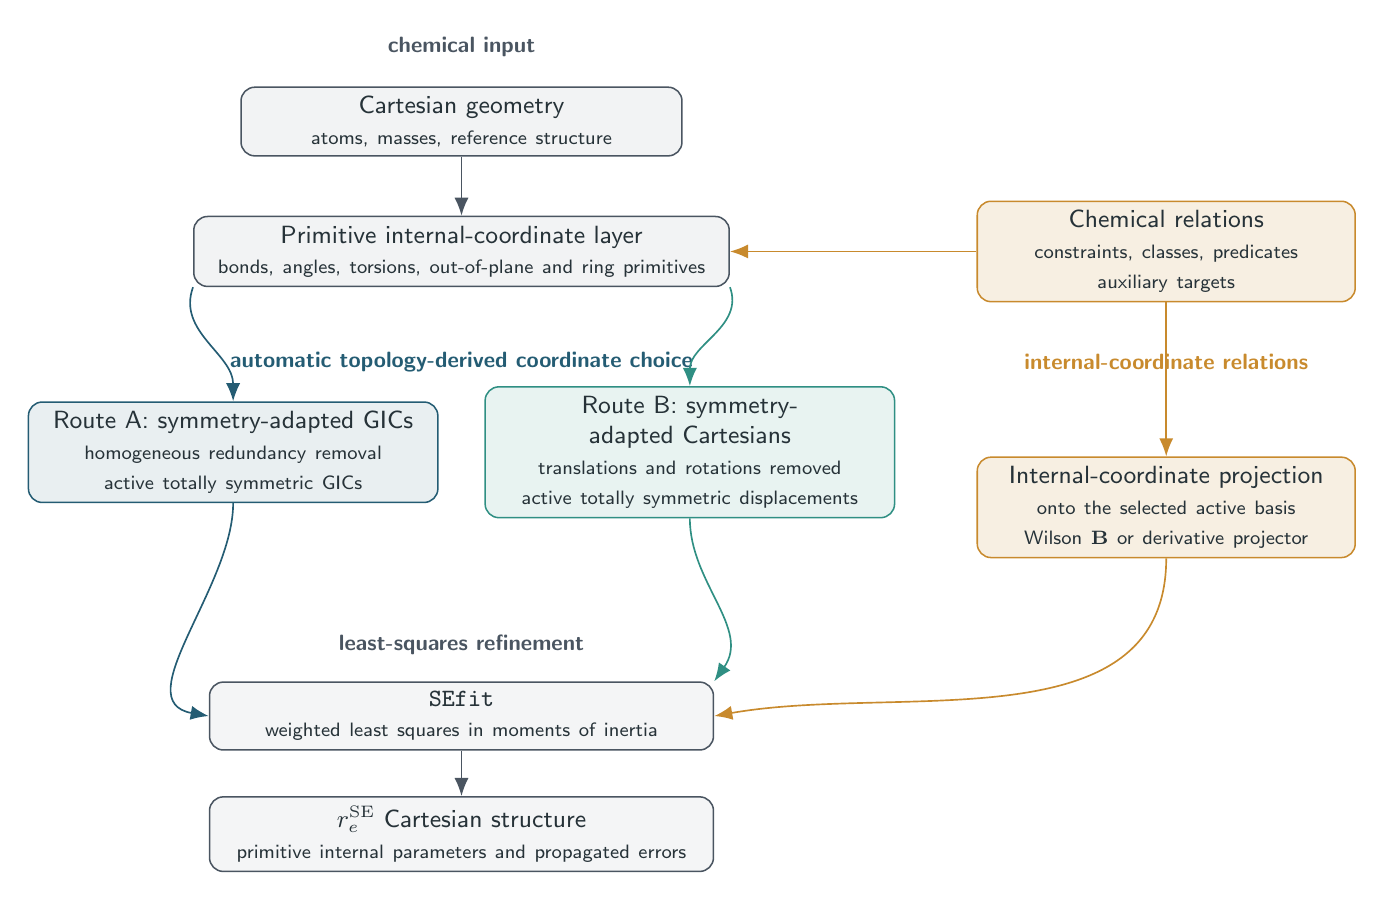
\begin{tikzpicture}[
  x=1cm,
  y=1cm,
  font=\sffamily\small,
  box/.style={
    draw,
    rounded corners=5pt,
    align=center,
    minimum height=0.82cm,
    line width=0.55pt,
    text=MerlinoInk,
    fill=white
  },
  inputbox/.style={box, fill=MerlinoSlate!7, draw=MerlinoSlate, minimum width=5.6cm, text width=5.2cm},
  primbox/.style={box, fill=MerlinoSlate!7, draw=MerlinoSlate, minimum width=6.8cm, text width=6.4cm},
  gicbox/.style={box, fill=MerlinoBlue!10, draw=MerlinoBlue, minimum width=5.2cm, text width=4.9cm},
  cartbox/.style={box, fill=MerlinoTeal!11, draw=MerlinoTeal, minimum width=5.2cm, text width=4.9cm},
  sidebox/.style={box, fill=MerlinoGold!14, draw=MerlinoGold, minimum width=4.8cm, text width=4.4cm},
  outbox/.style={box, fill=MerlinoSlate!6, draw=MerlinoSlate, minimum width=6.4cm, text width=6.0cm},
  arrow/.style={-{Latex[length=2.3mm,width=1.8mm]}, line width=0.60pt, draw=MerlinoSlate},
  gicarrow/.style={arrow, draw=MerlinoBlue},
  cartarrow/.style={arrow, draw=MerlinoTeal},
  sidearrow/.style={arrow, draw=MerlinoGold}
]
\node[font=\footnotesize\bfseries\sffamily, text=MerlinoSlate] at (-3.4,0.95) {chemical input};
\node[font=\footnotesize\bfseries\sffamily, text=MerlinoBlue] at (-3.4,-3.05) {automatic topology-derived coordinate choice};
\node[font=\footnotesize\bfseries\sffamily, text=MerlinoGold] at (5.55,-3.05) {internal-coordinate relations};
\node[font=\footnotesize\bfseries\sffamily, text=MerlinoSlate] at (-3.4,-6.65) {least-squares refinement};

\node[inputbox] (geom) at (-3.4,0) {Cartesian geometry\\{\scriptsize atoms, masses, reference structure}};
\node[primbox] (prim) at (-3.4,-1.65) {Primitive internal-coordinate layer\\{\scriptsize bonds, angles, torsions, out-of-plane and ring primitives}};
\node[sidebox] (relations) at (5.55,-1.65) {Chemical relations\\{\scriptsize constraints, classes, predicates}\\{\scriptsize auxiliary targets}};

\node[gicbox] (gicroute) at (-6.3,-4.20) {Route A: symmetry-adapted GICs\\{\scriptsize homogeneous redundancy removal}\\{\scriptsize active totally symmetric GICs}};
\node[cartbox] (cartroute) at (-0.5,-4.20) {Route B: symmetry-adapted Cartesians\\{\scriptsize translations and rotations removed}\\{\scriptsize active totally symmetric displacements}};
\node[sidebox] (project) at (5.55,-4.90) {Internal-coordinate projection\\{\scriptsize onto the selected active basis}\\{\scriptsize Wilson $\mathbf{B}$ or derivative projector}};
\node[outbox] (sefit) at (-3.4,-7.55) {\texttt{SEfit}\\{\scriptsize weighted least squares in moments of inertia}};
\node[outbox] (result) at (-3.4,-9.05) {$r_e^{\mathrm{SE}}$ Cartesian structure\\{\scriptsize primitive internal parameters and propagated errors}};

\draw[arrow] (geom) -- (prim);
\draw[sidearrow] (relations.west) -- (prim.east);
\draw[gicarrow] (prim.south west) to[out=-110,in=90] (gicroute.north);
\draw[cartarrow] (prim.south east) to[out=-70,in=90] (cartroute.north);
\draw[sidearrow] (relations.south) -- (project.north);
\draw[gicarrow] (gicroute.south) to[out=-90,in=170] (sefit.west);
\draw[cartarrow] (cartroute.south) to[out=-90,in=55] (sefit.north east);
\draw[sidearrow] (project.south) to[out=-90,in=10] (sefit.east);
\draw[arrow] (sefit) -- (result);
\end{tikzpicture}
}
\caption{Architecture of the automatic \texttt{SEfit}
workflow. Cartesian geometry defines topology and primitive internal
coordinates once. The active least-squares space is then chosen as either
Route A, a non-redundant symmetry-adapted GIC basis, or Route B, a
symmetry-adapted Cartesian basis with translations and rotations removed.
Constraints, parameter classes, and predicates remain internal-coordinate
objects and are projected onto either active basis before refinement. The final
Cartesian structure and the propagated errors of primitive internal parameters
are generated by the same reporting layer. Auxiliary model information is
handled in the chemical-relation layer and is not inserted into the covalent
graph used to generate GICs.}
\label{fig:workflow-architecture}
\end{figure*}

This separation between chemical specification, active coordinate basis, and
least-squares refinement allows the same infrastructure to support both
semiexperimental structure determination and other coordinate-dependent
modules.


\subsection{Primitive Coordinate Generation}

The coordinate construction starts from a Cartesian molecular geometry.
The coordinate engine first perceives the covalent graph, including bonded atom
pairs and ring connectivity. This graph is the only topology used for
primitive-coordinate generation, ring detection, redundancy removal, and
symmetry adaptation.

The graph is then expanded into a deliberately redundant primitive set:
stretches, valence angles, torsions, out-of-plane deformations, linear bends,
and ring-specific primitives. Redundancy at this stage is useful because it
preserves locality and avoids forcing a premature choice of which primitive
coordinates should become fitted variables.

Auxiliary reference information is kept outside the covalent graph. It may
define constraints, predicates, or starting-geometry corrections, but it is not
inserted into primitive GIC generation or ring detection.

For cyclic systems, ring coordinates are generated from endocyclic torsions and
from analogous combinations of endocyclic valence angles. Unlike
Cremer--Pople variables\cite{CremerPople1975} or manually defined ring
coordinates, these primitives remain within the generalized-internal-coordinate
formalism and are available for monocyclic, fused-ring, bridged, and
polycyclic systems.

This primitive layer is also the user-facing chemical interface. Constraints,
predicates, and parameter classes are expressed here and remain independent of
the non-redundant active representation generated later.


\subsection{Coordinates for Parameter Refinement}

Refinement coordinates must define statistical parameters, not merely a
convenient optimization path. The normal matrix must have a controlled rank,
the covariance matrix must be interpretable, and the resulting uncertainty
must be propagated to reported bond lengths, angles, dihedrals, and other
derived quantities. The active space is therefore required to be
non-redundant, symmetry consistent, and compatible with chemically meaningful
constraints.

This requirement exposes the non-uniqueness of Z-matrices. A Z-matrix selects
a rooted traversal of the molecular graph. For rings, fused systems, and
bridged skeletons, no traversal can make all chemically equivalent edges
primary at the same time; at least one ring-closing distance or related
quantity is derived. The fitted covariance is then attached to the chosen
coordinate model as well as to the molecule.

Two active spaces are used here. In the GIC route, all topologically implied
primitive internals are generated first and then reduced and symmetry adapted
within homogeneous families, so stretches, bends, torsions, out-of-plane
motions, and ring coordinates do not replace one another during rank
reduction.\cite{PulayFogarasi1992,Peng1996Redundant,Baker1996Delocalized,BakkenHelgaker2002}
In the Cartesian route, translations and rotations are removed directly from
the Cartesian displacement space and the totally symmetric block is retained.
Both routes start from the same Cartesian geometry, use the same
primitive-coordinate constraint layer, and report the same final structural
observables with propagated uncertainties.

Symmetry both restricts the active variables to the totally symmetric
representation and completes primitive constraints over equivalent orbits.
Non-totally-symmetric coordinates remain available for diagnostics but are
inactive in an equilibrium refinement.


\subsection{Non-Redundant Symmetry-Adapted GICs}

The primitive-coordinate set generated from topology is chemically intuitive
but redundant. Linear dependencies from graph connectivity, ring closure, and
symmetry are removed before refinement so that the normal equations and
covariance matrix are defined in an independent coordinate space.

Let $\mathbf{x}\in \mathbb{R}^{3N}$ be the Cartesian coordinate vector and let

\begin{equation}
\mathbf{s}(\mathbf{x}) =
(s_1(\mathbf{x}),s_2(\mathbf{x}),\ldots,s_m(\mathbf{x}))^T
\end{equation}

collect the primitive internal coordinates. At a reference geometry
$\mathbf{x}_0$, primitive displacements and Cartesian displacements are
related to first order by the Wilson matrix\cite{Wilson1955}

\begin{equation}
\Delta \mathbf{s}
=
\mathbf{B}_s
\Delta \mathbf{x},
\qquad
\mathbf{B}_s =
\left.
\frac{\partial \mathbf{s}}
{\partial \mathbf{x}}
\right|_{\mathbf{x}_0}.
\end{equation}

The primitive vector is partitioned into homogeneous families,

\begin{equation}
\mathbf{s}
=
\left(
\mathbf{s}_{\mathrm{str}},
\mathbf{s}_{\mathrm{bend}},
\mathbf{s}_{\mathrm{tor}},
\mathbf{s}_{\mathrm{oop}},
\mathbf{s}_{\mathrm{ring}},
\ldots
\right),
\end{equation}

Reduction to non-redundant GICs precedes symmetry adaptation and is performed
with a rank-revealing transformation of the full primitive set. Blocks are
processed in fixed topological order with common singular-value thresholds.
For each coordinate family $\alpha$, the Wilson block is

\begin{equation}
\mathbf{B}_{s_\alpha}
=
\frac{\partial\mathbf{s}_\alpha}
{\partial\mathbf{x}} .
\end{equation}

A singular-value decomposition,\cite{GolubReinsch1970}

\begin{equation}
\mathbf{B}_{s_\alpha}
=
\mathbf{U}_{\alpha}
\boldsymbol{\Sigma}_{\alpha}
\mathbf{V}_{\alpha}^{T},
\end{equation}

identifies the independent primitive-coordinate differential space. Retained
left-singular vectors define the row-orthonormal transformation

\begin{equation}
\mathbf{R}_{\alpha}
=
\mathbf{U}_{\alpha,r}^{T},
\end{equation}

where the subscript $r$ denotes the retained singular subspace. The
non-redundant coordinates for family $\alpha$ are then

\begin{equation}
\Delta \mathbf{q}_\alpha
=
\mathbf{R}_\alpha
\Delta \mathbf{s}_\alpha ,
\qquad
\mathbf{B}_{q_\alpha}
=
\mathbf{R}_\alpha
\mathbf{B}_{s_\alpha}.
\end{equation}

The number of retained coordinates is the rank of
$\mathbf{B}_{s_\alpha}$. If the stretching block is already full rank,
primitive stretches are retained unchanged; other blocks are reduced only
within the same physical family.

Stacking the blocks gives

\begin{equation}
\Delta \mathbf{q}
=
\mathbf{R}
\Delta \mathbf{s},
\qquad
\mathbf{B}_{q}
=
\mathbf{R}
\mathbf{B}_s .
\end{equation}

The block-diagonal structure of $\mathbf{R}$ preserves chemical homogeneity:
rank reduction cannot use one coordinate family to replace another. After the
family-wise reduction, $\mathbf{B}_q$ is checked against the expected
vibrational rank. Any residual dependencies are pruned with the family blocks
kept explicit and deterministic topological tie breaking. Molecular symmetry
is applied only after this unsymmetrized non-redundant basis has been fixed.

Symmetry is then applied to the non-redundant GIC space. For each operation
$g$ of the detected point group, the coordinate engine constructs the induced
operation $\mathbf{D}_q(g)$ on $\Delta\mathbf{q}$ from the atom permutation,
Cartesian rotation, and primitive-coordinate transformation. The projector
onto irreducible representation $\Gamma$ is

\begin{equation}
\mathbf{P}^{q}_{\Gamma}
=
\frac{d_{\Gamma}}{|G|}
\sum_{g\in G}
\chi_{\Gamma}(g)
\mathbf{D}_q(g),
\end{equation}

where $d_{\Gamma}$ and $\chi_{\Gamma}$ are the dimension and character of
$\Gamma$. Orthonormal columns of $\mathbf{S}_{\Gamma}$ span the range of this
projector, and the symmetry-adapted GICs are

\begin{equation}
\Delta \mathbf{Q}_{\Gamma}
=
\mathbf{S}_{\Gamma}^{T}
\Delta \mathbf{q}.
\end{equation}

Only the totally symmetric block is active in an equilibrium refinement,

\begin{equation}
\Delta \mathbf{Q}
\equiv
\Delta \mathbf{Q}_{A_1}
=
\mathbf{S}_{A_1}^{T}
\mathbf{R}
\Delta \mathbf{s}
=
\mathbf{B}_{Q}
\Delta \mathbf{x},
\end{equation}

with

\begin{equation}
\mathbf{B}_{Q}
=
\mathbf{S}_{A_1}^{T}
\mathbf{R}
\mathbf{B}_s .
\end{equation}

Cartesian displacements associated with GIC corrections use the
rank-controlled minimum-norm solution

\begin{equation}
\Delta \mathbf{x}
=
\mathbf{B}_{Q}^{+}
\Delta \mathbf{Q},
\end{equation}

where the Moore--Penrose pseudoinverse uses explicit singular-value
thresholds and topology validation after accepted steps. For geometry
corrections from target internal coordinates, the same derivative machinery
can be used in weighted form by minimizing

\begin{equation}
\left\|
\mathbf{W}_{s}^{1/2}
\left(
\mathbf{B}_{t}\Delta\mathbf{x}
-
\Delta\mathbf{t}
\right)
\right\|^2 ,
\end{equation}

where $\mathbf{t}$ contains requested internal-coordinate changes or auxiliary
reference targets. The diagonal metric $\mathbf{W}_{s}$ assigns different
stiffness to coordinate families; auxiliary targets are not part of the
covalent GIC active space unless a dedicated block is defined.


\subsection{Symmetry-Adapted Cartesian Coordinates}

The same least-squares machinery can also operate in a symmetry-adapted
Cartesian displacement basis. This gives a direct Cartesian update route while
retaining the same symmetry selection, constraint projection, and covariance
propagation used for GICs.

Starting from the reference geometry, external translations and rotations are
removed. Let $\mathbf{E}\in\mathbb{R}^{3N\times n_{\mathrm{ext}}}$ collect
these vectors, with $n_{\mathrm{ext}}=6$ for a nonlinear molecule and
$n_{\mathrm{ext}}=5$ for a linear one. Rotational columns are generated from
infinitesimal rotations around the center of mass,

\begin{equation}
\Delta\mathbf{r}_i
=
\boldsymbol{\omega}
\times
\left(
\mathbf{r}_i-\mathbf{r}_{\mathrm{cm}}
\right),
\end{equation}

for each atom $i$. The columns of $\mathbf{E}$ are orthonormalized to give
$\mathbf{Z}_{\mathrm{ext}}$, and the internal Cartesian projector is

\begin{equation}
\mathbf{P}_{\mathrm{vib}}
=
\mathbf{I}_{3N}
-
\mathbf{Z}_{\mathrm{ext}}
\mathbf{Z}_{\mathrm{ext}}^{T}.
\end{equation}

This projector defines the non-redundant Cartesian displacement space before
symmetry classification.

For each irreducible representation $\Gamma$ of the automatically detected
point group, a Cartesian symmetry projector is constructed directly in the
$3N$-dimensional displacement space as

\begin{equation}
\mathbf{P}^{x}_{\Gamma}
=
\frac{d_{\Gamma}}{|G|}
\sum_{g\in G}
\chi_{\Gamma}(g)
\mathbf{R}(g),
\end{equation}

where $\mathbf{R}(g)$ is the Cartesian operation, including atom permutation,
associated with the symmetry operation $g$. Orthonormal columns spanning
$\mathbf{P}_{\mathrm{vib}}\mathbf{P}^{x}_{\Gamma}\mathbf{P}_{\mathrm{vib}}$
define the symmetry-adapted Cartesian basis,

\begin{equation}
\mathrm{range}
\left(
\mathbf{P}_{\mathrm{vib}}
\mathbf{P}^{x}_{\Gamma}
\mathbf{P}_{\mathrm{vib}}
\right)
=
\mathrm{span}
\left(
\mathbf{C}_{\Gamma}
\right).
\end{equation}

The columns of $\mathbf{C}_{\Gamma}$ are orthonormal displacement directions,
not force-field normal modes. Only the totally symmetric block is used,

\begin{equation}
\Delta \mathbf{x} =
\mathbf{C}_{A_1}
\Delta \mathbf{q}_{\mathrm{SC}},
\end{equation}

where $\Delta \mathbf{q}_{\mathrm{SC}}$ are amplitudes along the totally
symmetric Cartesian directions. Primitive variations induced by these
amplitudes are

\begin{equation}
\Delta \mathbf{s}
=
\mathbf{B}_s
\mathbf{C}_{A_1}
\Delta \mathbf{q}_{\mathrm{SC}} .
\end{equation}

This links the Cartesian active space to the same primitive-coordinate
interface used by GICs. Bonds, angles, local hydrogen constraints, and
Gaussian-style \texttt{ModRedundant} freezes are still specified as internal
relations and projected by $\mathbf{B}_s\mathbf{C}_{A_1}$. Direct Cartesian
constraints are avoided because a fixed bond or angle is a nonlinear,
orientation-free relation distributed over several Cartesian components. Final
bond lengths, valence angles, dihedrals, and uncertainties are evaluated from
the optimized Cartesian geometry, as in the GIC route.


\subsection{Constraints, Predicates, and Parameter Classes}

User-defined structural relations are specified in primitive internal
coordinates,

\begin{equation}
\mathbf{s} = (s_1,s_2,\ldots,s_m)^T ,
\end{equation}

not in GIC amplitudes or Cartesian components. The same primitive relation is
projected onto either active space. Let $\Delta\mathbf{a}$ be the active
correction vector. For GICs, $\Delta\mathbf{a}=\Delta\mathbf{Q}$ and

\begin{equation}
\Delta\mathbf{x}
=
\mathbf{T}_{A}\Delta\mathbf{a},
\qquad
\mathbf{T}_{A}=\mathbf{B}_{Q}^{+}.
\end{equation}

For symmetry Cartesians, $\Delta\mathbf{a}=\Delta\mathbf{q}_{\mathrm{SC}}$ and

\begin{equation}
\Delta\mathbf{x}
=
\mathbf{T}_{A}\Delta\mathbf{a},
\qquad
\mathbf{T}_{A}=\mathbf{C}_{A_1}.
\end{equation}

Primitive corrections induced by any active coordinate model are therefore

\begin{equation}
\Delta\mathbf{s}
=
\mathbf{B}_s
\mathbf{T}_{A}
\Delta\mathbf{a}.
\end{equation}

This projector is used for constraints, predicates, classes, and error
propagation.

\paragraph{Hard constraints.}

Hard constraints are exact equations imposed throughout the refinement:

\begin{equation}
s_i=s_i^{0},
\end{equation}

equalities,

\begin{equation}
s_i-s_j=0,
\end{equation}

or general linearized functions,

\begin{equation}
\mathbf{c}(\mathbf{s})=\mathbf{d}.
\end{equation}

At a trial geometry the corresponding first-order condition is

\begin{equation}
\mathbf{C}_s
\Delta\mathbf{s}
=
\mathbf{b}_c,
\qquad
\mathbf{C}_s =
\left.
\frac{\partial\mathbf{c}}
{\partial\mathbf{s}}
\right|_{\mathbf{s}_0},
\qquad
\mathbf{b}_c=\mathbf{d}-\mathbf{c}(\mathbf{s}_0).
\end{equation}

Projection to the active space gives

\begin{equation}
\mathbf{C}_{A}
\Delta\mathbf{a}
=
\mathbf{b}_c,
\qquad
\mathbf{C}_{A}
=
\mathbf{C}_s
\mathbf{B}_s
\mathbf{T}_{A}.
\end{equation}

The solver keeps all compatible motions by writing the allowed correction as

\begin{equation}
\Delta\mathbf{a}
=
\Delta\mathbf{a}_0
+
\mathbf{N}\Delta\mathbf{p},
\qquad
\mathbf{C}_{A}\mathbf{N}=\mathbf{0},
\end{equation}

where $\Delta\mathbf{a}_0$ is a minimum-norm particular solution and
$\mathbf{N}$ spans the null space. The least-squares problem is solved only
for $\Delta\mathbf{p}$.

Symmetry-equivalent primitives are constrained as complete orbits before the
null-space projector is formed. Gaussian-style \texttt{ModRedundant} freezes
and generalized-internal-coordinate expressions are interpreted in this
primitive layer. A line \texttt{Name=Expression} defines a reusable coordinate;
\texttt{Frozen,Value=} turns it into a hard equation. Names can combine
stretches, angles, dihedrals, out-of-plane coordinates, Cartesian components,
or final \texttt{GIC}\emph{n} labels. If \texttt{Value=} is omitted, the
starting-geometry value is frozen; tabulated structural information therefore
uses explicit \texttt{Value=} targets.

Reduced-dimensionality refinements use the same projection. Hydrogen
coordinates supported by isotopic data remain refinable, whereas unsupported
local hydrogen frames can be frozen or tied without over-constraining the
heavy-atom skeleton. Additional model-dependent geometry information is kept
outside the covalent topology used for GIC generation.

\paragraph{Predicate observations.}

Predicates are soft structural information. They add weighted residuals rather
than removing degrees of freedom.\cite{Bartell1975Predicate} A primitive
predicate has the form

\begin{equation}
f(\mathbf{s})
=
f^{\mathrm{ref}}
\pm
\sigma_f ,
\end{equation}

and contributes

\begin{equation}
r_f
=
\frac{f(\mathbf{s})-f^{\mathrm{ref}}}{\sigma_f}
\end{equation}

to the residual vector. Its Jacobian with respect to the independent
least-squares variables is

\begin{equation}
\mathbf{J}_f
=
\frac{1}{\sigma_f}
\frac{\partial f}{\partial\mathbf{s}}
\mathbf{B}_s
\mathbf{T}_{A}
\mathbf{N}.
\end{equation}

Their uncertainties control their statistical weight.

\paragraph{Parameter classes.}

Parameter classes make several primitive quantities share one correction. If
class $c$ contains primitives $i\in c$, the allowed correction is

\begin{equation}
\Delta s_i
=
\Delta p_c,
\qquad
i\in c .
\end{equation}

Class definitions are converted into linear relations or into a Jacobian
compression before the normal equations are solved. The operation applies to
corrections rather than final values, so chemically related quantities may
retain different reference values while sharing a fitted offset. After
convergence, the covariance is expanded back to the reported primitive and
topological parameters.


\subsection{Semiexperimental Observables}

For each isotopologue $s$, the measured ground-state rotational constants are
converted into equilibrium rotational constants by removing vibrational and,
when necessary, electronic contributions,\cite{Costain1958,Pawlowski2002,Piccardo2015B3LYP,Penocchio2015B2PLYP}

\begin{equation}
B_{\alpha,e}^{(s)}
= B_{\alpha,0}^{(s)}
- \Delta B_{\alpha,\mathrm{vib}}^{(s)}
- \Delta B_{\alpha,\mathrm{elec}}^{(s)},
\qquad
\alpha \in \{a,b,c\}.
\end{equation}

The correction terms may come from any electronic-structure or composite
protocol and are supplied through the isotopologue data file together with
uncertainties, masses, conventions, and provenance.\cite{Mendolicchio2025FastDvib}

Although rotational constants may be fitted directly, \texttt{SEfit} uses
principal moments of inertia as the default observables,

\begin{equation}
I_{\alpha}^{(s)}
=
\frac{K}
{B_{\alpha,e}^{(s)}},
\end{equation}

where $K$ is the standard rotational conversion constant.

Moments of inertia give a smoother geometry dependence and avoid reciprocal
amplification of small constant variations.

Rotational constants can still be fitted for diagnostics. For planar
molecules, however, only two principal components are independent. If the
molecular plane is the $ab$ plane,

\begin{equation}
I_c = I_a + I_b ,
\end{equation}

Fitting all three components would duplicate one constraint. \texttt{SEfit}
therefore uses one pair, $AB$, $AC$, or $BC$, and reports the omitted
component as a diagnostic. Planarity is recognized from the singular values of
the centered Cartesian geometry. If the user does not choose a pair, the code
tests all admissible pairs, keeps the largest numerical rank, and among
rank-equivalent choices minimizes the propagated instability of the omitted
moment from the planar identity. The Jacobian condition number is only the
final tie-breaker; forced $ABC$ planar fits are rejected as redundant.

The complete experimental data set consists of the selected observables for all
isotopologues and their uncertainties. These values form the experimental part
of the least-squares objective described below.


\subsection{Least-Squares Refinement}

The semiexperimental refinement is formulated as a weighted nonlinear
least-squares problem. The active coordinate vector $\mathbf{a}$ is either the
totally symmetric GIC vector or the totally symmetric Cartesian displacement
amplitude vector. After hard constraints and parameter classes have been
projected, the actual independent least-squares variables are collected in
$\mathbf{p}$.

The residual vector is

\begin{equation}
\mathbf{r}
= \mathbf{y}^{\mathrm{obs}}
- \mathbf{y}^{\mathrm{calc}}(\mathbf{p}),
\end{equation}

where $\mathbf{y}$ collects all experimental observables and predicate
observations included in the refinement.

The objective function is

\begin{equation}
\chi^2
=
\mathbf{r}^{T}
\mathbf{W}
\mathbf{r},
\end{equation}

where $\mathbf{W}$ is the diagonal weight matrix constructed from the inverse
variances of the experimental and predicate observations.
When robust fitting is requested, the experimental part of $\mathbf{W}$ is
modified by an iteratively reweighted loss applied to complete isotopologue
blocks rather than to individual rotational constants. Thus all selected
components of a suspect isotopologue are attenuated together, whereas
quantum-chemical predicates retain their assigned statistical weights.

The optimization is performed using a weighted Levenberg--Marquardt procedure,

\begin{equation}
\left(
\mathbf{J}^{T}
\mathbf{W}
\mathbf{J}
+
\lambda \mathbf{I}
\right)
\Delta \mathbf{p}
=
\mathbf{J}^{T}
\mathbf{W}
\mathbf{r},
\label{eq:lm-step}
\end{equation}

where $\mathbf{J}$ is the Jacobian matrix of the observables with respect to
the independent variables $\mathbf{p}$ and $\lambda$ is the damping parameter.
Equation~\eqref{eq:lm-step} is not solved in the implementation by forming
normal equations. The Python driver solves the corresponding column-scaled
trust-region subproblem in singular-value-decomposition (SVD) coordinates:
the rank-revealing Gauss--Newton step is used when it lies inside the current
trust radius, whereas an active-radius step is obtained by determining the
Levenberg shift from the More--Hebden secular equation. QR solution of the
augmented Levenberg--Marquardt system and Cauchy steps are retained as
fallbacks.\cite{GolubReinsch1970} The
diagonal scaling matrix $\mathbf{S}$ is updated from the current weighted
Jacobian column norms, on top of the chemical coordinate-family scaling. This
prevents weakly observed variables or mixed units from controlling the
trust-region step and avoids the condition-number squaring associated with
explicit normal equations.

The Jacobian is evaluated analytically whenever possible. Independent
coordinate corrections are transformed into active-coordinate corrections,
then into Cartesian displacements through the projector
$\mathbf{T}_{A}\mathbf{N}$ described above. This gives analytic derivatives of
moments of inertia and rotational constants with respect to the variables that
are actually fitted.

The solver uses a trust-region Levenberg--Marquardt strategy based on the
predicted and actual reduction of the weighted objective
function.\cite{More1978LevenbergMarquardt} Trial line-search points are
evaluated with a frozen coordinate model. Every accepted step is then validated
by the coordinate-definition service against the original topology, point group,
irreducible-representation counts, and coordinate-family counts. Steps that
would change this GIC signature are rejected and the trust radius is reduced.
The Cartesian--GIC projector is refreshed analytically when needed and
otherwise updated by a secant correction, avoiding unnecessary coordinate
rebuilds without accepting topology-changing steps.
The independent Fortran77 numerical-kernel layer provides dynamic column
scaling, rank-revealing QR solution of the augmented Levenberg--Marquardt
system, and grouped robust weights without importing legacy Gaussian code.

Convergence requires both the parameter corrections and the objective-function
reduction to fall below predefined thresholds. Trial steps that increase the
objective are rejected automatically, and the damping parameter is adjusted
adaptively.
For validation, \texttt{SEfit} can perform exact leave-one-isotopologue-out
refits. Each isotopologue is removed in turn, the geometry is refitted with the
same coordinate and constraint model, and the omitted rotational constants are
predicted from the resulting structure. These diagnostics are not part of the
objective function; they identify outlier isotopologues and quantify how
strongly individual substitutions control the fitted geometry.
The same philosophy is used for numerical warnings: reduced rank, small
singular values, strongly downweighted isotopologues, ill-conditioned planar
component pairs, and unusually large propagated coordinate uncertainties are
reported explicitly, but they do not redefine the coordinate model or the
least-squares objective.

Following convergence, the covariance matrix in the independent fitted
variables is obtained from

\begin{equation}
\mathbf{C}_{p}
=
\sigma_r^2
\left(
\mathbf{J}^{T}
\mathbf{W}
\mathbf{J}
\right)^{-1},
\end{equation}

where $\sigma_r^2$ is the reduced residual variance.

\subsection{Error Propagation}

Uncertainty propagation follows the same chain of transformations used for the
geometry update. If $\mathbf{N}$ is the null-space basis of the hard
constraints and class reductions, the covariance in the active coordinate
space is

\begin{equation}
\mathbf{C}_{a}
=
\mathbf{N}
\mathbf{C}_{p}
\mathbf{N}^{T}.
\end{equation}

The corresponding Cartesian covariance is

\begin{equation}
\mathbf{C}_{x}
=
\mathbf{T}_{A}
\mathbf{C}_{a}
\mathbf{T}_{A}^{T}.
\end{equation}

For a GIC refinement, $\mathbf{T}_{A}=\mathbf{B}_{Q}^{+}$; for a Cartesian
refinement, $\mathbf{T}_{A}=\mathbf{C}_{A_1}$. Therefore the same covariance
propagation is used for both coordinate choices.

Any reported structural quantity is treated as a function of the optimized
Cartesian geometry. For a vector of reported quantities
$\mathbf{g}(\mathbf{x})$, which may contain bond lengths, valence angles,
dihedral angles, out-of-plane coordinates, ring descriptors, or user-defined
primitive functions, the covariance is

\begin{equation}
\mathbf{C}_{g}
=
\mathbf{G}_{x}
\mathbf{C}_{x}
\mathbf{G}_{x}^{T},
\qquad
\mathbf{G}_{x}
=
\left.
\frac{\partial\mathbf{g}}
{\partial\mathbf{x}}
\right|_{\mathbf{x}_{\mathrm{opt}}}.
\end{equation}

The reported standard errors are the square roots of the diagonal elements of
$\mathbf{C}_{g}$, while the off-diagonal elements provide correlations among
derived structural parameters. Angular derivatives are evaluated in radians
and converted to degrees only in the final report. Symmetry-equivalent
reported quantities can either be listed separately with their covariance or
condensed by the same linear propagation formula.

Hard constraints have no variance along the constrained directions because
those directions are removed before the normal equations are solved. Predicate
observations are different: their stated uncertainties enter the weight matrix
and therefore contribute statistically to $\mathbf{C}_{p}$. This distinction is
important when hydrogen parameters are held fixed because deuterated
isotopologues are unavailable. A frozen local hydrogen frame is a constraint;
a quantum-chemical C--H distance with an assigned uncertainty is a predicate.
Only the latter contributes uncertainty through its assigned standard
deviation.

The output therefore reports both standard errors and correlation diagnostics.
Large correlations are not treated as failures by themselves, because they are
expected whenever isotope substitutions do not isolate all local structural
directions. They are used to identify underdetermined parameter combinations,
to decide whether a primitive should be fixed or converted into a predicate,
and to verify that reported derived quantities are propagated from the full
covariance matrix rather than from independent one-parameter estimates.
The same information is complemented by an SVD diagnostic of the final weighted
Jacobian. Small singular values are reported together with the dominant
coordinate combinations in the corresponding right singular vectors, so a rank
deficiency can be traced to specific GICs, parameter classes, or
symmetry-Cartesian directions instead of being summarized only by a condition
number.

All constraints are also audited after projection. The output records the input
primitive patterns, the symmetry-equivalent primitive constraints generated from
them, the parameter classes, and the active working-coordinate labels actually
matched by each entry. This is important for black-box refinements: the user
does not construct the active coordinate basis manually, but can verify exactly
which chemically stated restrictions were imposed on that basis.

The final structural tables are thus independent of the internal coordinate
basis used during optimization. The fitted variables may be GIC amplitudes or
Cartesian amplitudes, but bond lengths, angles, dihedrals, and ring parameters
are always evaluated from the same optimized Cartesian geometry and receive
errors from the same propagated covariance matrix.

After convergence, \texttt{SEfit} also evaluates the numerical Hessian of the
weighted least-squares objective with respect to the independent variables that
remain after symmetry selection, parameter-class reduction, and constraint
projection. Diagonalization of this optimized-space Hessian provides the final
stationary-point diagnostic: a positive spectrum identifies a local minimum in
the fitted coordinate space, negative eigenvalues flag an unstable direction,
and near-zero eigenvalues are reported as rank-deficient or statistically flat
directions rather than hidden by the refinement. The benchmark tables therefore
report the stationary-point classification, and, where useful, the smallest
Hessian eigenvalue.


\subsection{Kraitchman Diagnostic}

For singly substituted isotopologues, \texttt{SEfit} computes substitution
coordinates from the Kraitchman equations\cite{Kraitchman1953} and compares
their absolute values with the fitted coordinates in the parent principal-axis
frame. This diagnostic is intentionally separate from the fit: Kraitchman
coordinates are useful assignment checks, but they do not retain coordinate
signs and do not exploit the full correlated least-squares model.


\section{Implementation and Reproducibility}

The implementation is organized around two reusable services. The coordinate-definition service
defines the molecular coordinate model from Cartesian atoms and nuclear
charges, assigning point-group symmetry and irreducible representations when
requested. A separate B-matrix service evaluates the same frozen GIC definition
for any compatible Cartesian geometry. \texttt{SEfit} calls the definition
service only at a fresh start and reuses the stored coordinate model during the
least-squares iterations, rebuilding or updating the B matrix only when the
current step requires it. The command-line interface and the graphical
interface call these same services and expose the choice between GIC and
symmetry-adapted Cartesian active spaces.

The standard input model contains Cartesian parent geometry, optional
Gaussian-style primitive freeze records, and a separate isotopologue file with
substitutions, ground-state rotational constants, vibrational and electronic
corrections, uncertainties, and correction conventions. Legacy MSR-style input
is accepted for reproducibility, including frozen variables marked by
\texttt{\#}, but it is converted immediately into the same Cartesian,
primitive-constraint, and isotopologue representation. Z-matrices are therefore
compatibility inputs, not working coordinates.

Each run writes a text report, final Cartesian coordinates, primitive internal
parameters with propagated uncertainties, corrected/calculated rotational
observables, residuals, covariance/correlation and influence diagnostics,
SVD, constraint, and warning diagnostics, Hessian eigenvalues for the minimum check,
Kraitchman diagnostics when applicable, and a machine-readable manifest. A
checkpoint file stores the Cartesian geometry, active labels, damping/trust
region state, and robust weights; restart calculations rebuild the GIC or
symmetry-Cartesian definitions deterministically from those Cartesian
coordinates. The benchmark tables in this article are generated from the
versioned run comma-separated-value (CSV) files by a single regression command, so the manuscript
values, test suite, and archived examples use the same numerical source. A
versioned distribution of the \texttt{SEfit} source code,
examples, and regression tests will be made available to reviewers and, upon
publication, under the distribution model selected by the authors.


\section{Relationship to Existing Approaches}

\texttt{SEfit} combines established semiexperimental least-squares
machinery\cite{Mendolicchio2017MSR,Bartell1975Predicate,Mendolicchio2025FastDvib}
with an automatically generated coordinate layer. The statistical model uses
moments of inertia, vibrational and electronic corrections, predicates,
parameter classes, leverage and correlation diagnostics, robust weighting, and
final minimum checks. The new element is not the observable model but the
definition of the refinement variables.

Z-matrices remain compact for tree-like molecules, as illustrated below by
glycolaldehyde. Their limitations become visible for rings, fused systems, and
bridged frameworks: a molecular graph with cycles cannot be represented by a
single reference tree without making some chemically equivalent quantities
primary and others derived. In a least-squares refinement this affects not
only notation but also the covariance attached to reported parameters.

Generalized internal coordinates are a flexible alternative and are widely
used in optimization and vibrational analysis.\cite{Wilson1955,PulayFogarasi1992,Peng1996Redundant,Baker1996Delocalized,BakkenHelgaker2002,Marenich2025GIC}
Gaussian, for example, provides a powerful GIC language for coordinate
combinations, constraints, scans, and conditional definitions.\cite{Peng1996Redundant,Marenich2025GIC}
In those workflows the generalized coordinates are usually a user-defined
layer. Here they are generated from topology-based primitive coordinates,
reduced to a non-redundant space, assigned to irreducible representations, and
accessed through primitive-coordinate constraints. Kisiel's
\texttt{STRFIT}/PROSPE route\cite{KisielPROSPE} provides another important
reference point for rotational-structure fitting, but the structural model is
again supplied by the user and may leave derived ring quantities outside the
primary fitted covariance matrix.\cite{Kanzow2025PCCP}

The practical distinction is summarized in Table~\ref{tab:workflow-comparison}.
\texttt{SEfit} retains the usual semiexperimental inputs and diagnostics while
moving coordinate construction, symmetry completion, and covariance propagation
to a common topology-derived layer.

\begin{table*}
\caption{Operational comparison of representative structure-refinement routes.
The table emphasizes coordinate construction and uncertainty reporting, not
the statistical quality of individual refinements.}
\label{tab:workflow-comparison}
\scriptsize
\setlength{\tabcolsep}{3pt}
\begin{tabular}{@{}>{\raggedright\arraybackslash}p{0.24\textwidth}>{\raggedright\arraybackslash}p{0.22\textwidth}>{\raggedright\arraybackslash}p{0.22\textwidth}>{\raggedright\arraybackslash}p{0.22\textwidth}@{}}
\toprule
Feature & Z-matrix semiexperimental workflows & User-defined GIC or \texttt{STRFIT}/PROSPE workflows & \texttt{SEfit} \\
\midrule
Primary geometry model & User-selected internal coordinates & User-supplied structural or generalized-coordinate model & Cartesian input with automatic topology perception \\
Ring and fused-ring treatment & Manual reference-tree choices & Manual parameter or coordinate selection & Automatic ring primitives and non-redundant active spaces \\
Symmetry handling & Specified in the chosen coordinate model & Defined by the supplied structural model & Automatic point-group detection and symmetry completion \\
Active variables & User-selected structural parameters & User-selected fitted parameters or GICs & Totally symmetric GICs or symmetry Cartesians \\
Constraints and classes & Expressed in the selected model & Expressed in the supplied model & Expressed as primitive internals and projected automatically \\
Missing substitution data & Reduced-dimensionality choices in the model & Fixed or selected parameters & Constraints, predicates, classes, or symmetry-complete local frames \\
Derived structural uncertainties & Propagated according to the selected coordinate model & Propagated according to the supplied fitted-parameter model & Propagated from the optimized Cartesian structure \\
Diagnostics & Established least-squares diagnostics & Diagnostics provided by the selected program and workflow & Rank, conditioning, robust weights, correlations, and leave-one-out checks \\
\bottomrule
\end{tabular}
\end{table*}


\section{Validation and Representative Applications}

The validation set was chosen to separate standard and non-standard coordinate
problems. Glycolaldehyde is a small acyclic molecule for which a traditional
Z-matrix is straightforward; it verifies that the automatic procedure does not
lose efficiency in a simple case. Glycine I and II test reduced-dimensionality
refinements at two levels of complexity: Gly-I retains C$_s$ symmetry and uses
four simple structural constraints, whereas Gly-II is treated without symmetry
and uses coupled functional constraints. Cyclopentadiene, nitrobenzene,
azulene, and norcamphor are more demanding because rings,
planar rotational redundancy, fused topology, bridged connectivity, and
missing deuterium substitutions force conventional workflows to choose derived
coordinates, fixed hydrogen models, or manually coupled parameters.

No molecule-specific coordinate code was introduced. In every benchmark the
input structure was Cartesian. The coordinate engine generated the coordinate
model, \texttt{SEfit} selected the totally symmetric active space, and any
constraints were supplied as primitive internal-coordinate relations. The same
constraint definitions were used when the active basis was changed from GICs
to symmetry-adapted Cartesians.

The regression suite additionally checks GIC generation for pyridine, uracil,
guanine, water, cyclopentadiene, nitrobenzene, and azulene. These tests verify point-group
assignment, non-redundant coordinate counts, and totally symmetric dimensions
independently of the semiexperimental fit.

The atom numbering used in structural tables and diagnostic discussions is
shown in Figure~\ref{fig:numbering}. The labels come directly from the
Cartesian input order and the perceived topology, so they match the numbering
used by the coordinate engine, \texttt{SEfit}, and the primitive-coordinate
constraints.

\begin{figure*}
\centering
\begin{minipage}{0.31\textwidth}
\centering
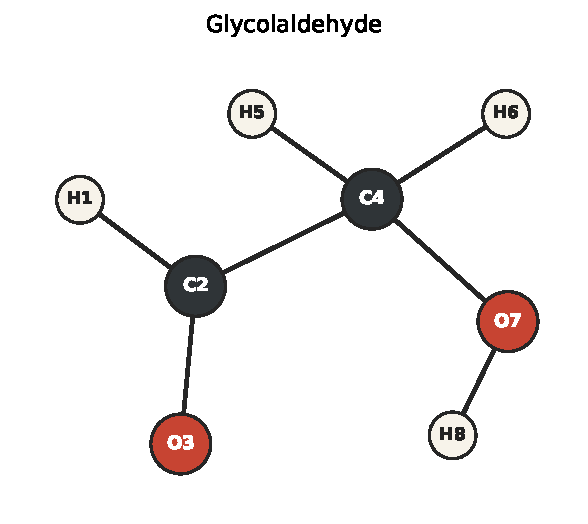
\includegraphics[width=\linewidth]{figures/glycolaldehyde_numbering.pdf}
\end{minipage}
\hfill
\begin{minipage}{0.31\textwidth}
\centering
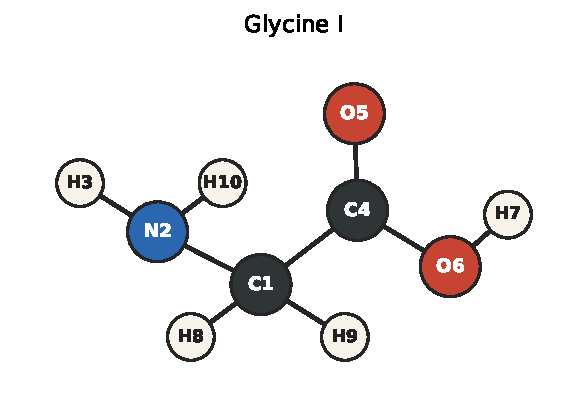
\includegraphics[width=\linewidth]{figures/glycine_I_numbering.pdf}
\end{minipage}
\hfill
\begin{minipage}{0.31\textwidth}
\centering
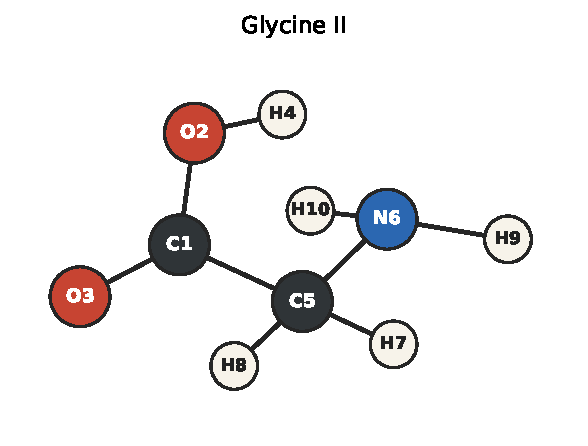
\includegraphics[width=\linewidth]{figures/glycine_II_numbering.pdf}
\end{minipage}

\vspace{0.6em}

\begin{minipage}{0.31\textwidth}
\centering
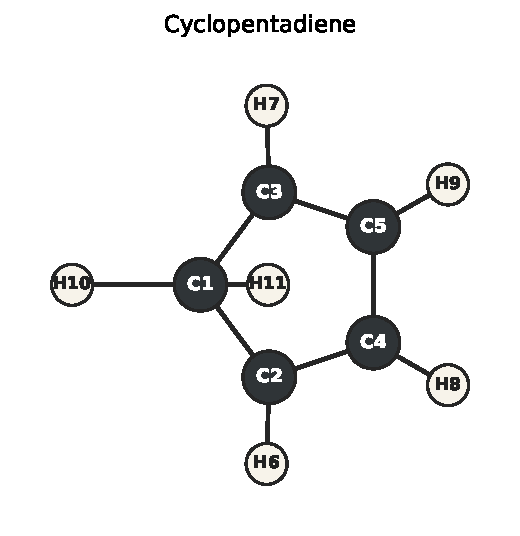
\includegraphics[width=\linewidth]{figures/cyclopentadiene_numbering.pdf}
\end{minipage}
\hfill
\begin{minipage}{0.31\textwidth}
\centering
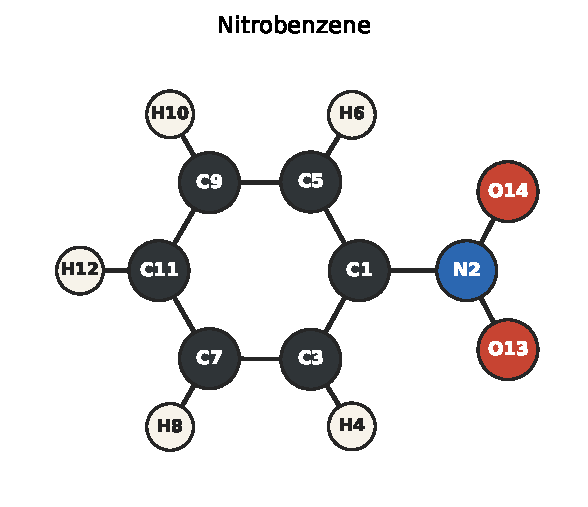
\includegraphics[width=\linewidth]{figures/nitrobenzene_numbering.pdf}
\end{minipage}
\hfill
\begin{minipage}{0.31\textwidth}
\centering
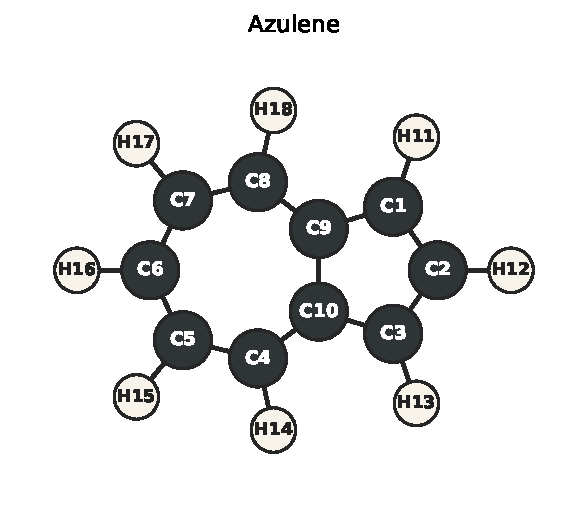
\includegraphics[width=\linewidth]{figures/azulene_numbering.pdf}
\end{minipage}

\vspace{0.6em}

\begin{minipage}{0.31\textwidth}
\centering
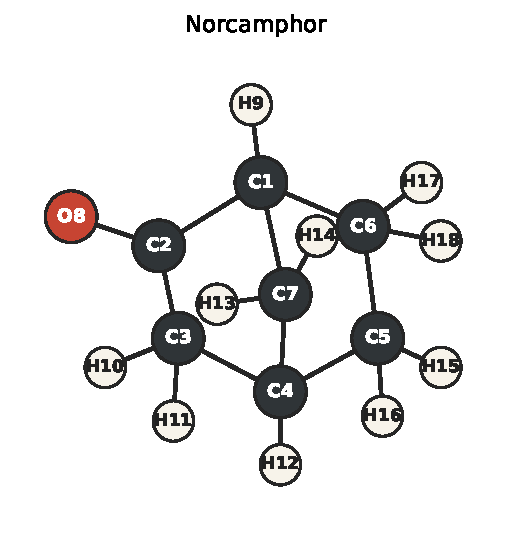
\includegraphics[width=\linewidth]{figures/norcamphor_numbering.pdf}
\end{minipage}
\caption{Atom numbering used for the glycolaldehyde, glycine I, glycine II, cyclopentadiene, nitrobenzene, azulene, and norcamphor semiexperimental refinements. The labels are derived from the Cartesian input order and are used consistently in the GIC definitions, primitive-coordinate constraints, and structural tables.}
\label{fig:numbering}
\end{figure*}

\input{generated/benchmark_summary.tex}

\input{generated/planar_pair_diagnostics.tex}

Table~\ref{tab:planar-pair-diagnostics} makes the planar choice explicit. The
selected $AB$ pair is not an arbitrary convention: it retains the two in-plane
moments directly and leaves the perpendicular constant as a diagnostic. Forced
$AC$ or $BC$ fits have the same rank but give larger complete rotational
diagnostic residuals for both nitrobenzene and azulene. In
Table~\ref{tab:benchmark-summary}, ``pos.'' denotes a rank-deficient statistical
Hessian with positive curvature in all retained fitted directions.

\subsection{Coordinate Content of the Benchmark Refinements}

The least-squares variables are not necessarily the topological quantities
listed in the final structural tables. They are either symmetry-adapted GICs or
symmetry-adapted Cartesian amplitudes. In both cases, reported bond lengths,
angles, dihedrals, and out-of-plane quantities are evaluated after convergence
from the optimized Cartesian geometry, with uncertainties propagated from the
fitted covariance matrix.

The primitive layer contains the local coordinates implied by the perceived
graph: stretches, valence angles, torsions, and ring deformation coordinates
derived from endocyclic valence-angle and torsional primitives. This redundant
set is reduced and symmetry-adapted in homogeneous blocks. Stretching GICs are
therefore formed only from stretches, valence-angle GICs only from
valence-angle primitives, and torsional or ring-puckering GICs only from
torsional-type primitives. This prevents a bond-stretching correction from
being replaced by a ring-puckering or torsional correction during rank
reduction.

The coordinate counts in Table~\ref{tab:coordinate-content} refer to the
covalent-topology GIC space. Auxiliary reference targets are deliberately not
included in these counts, because they do not create additional ring or GIC
primitives.

Table~\ref{tab:coordinate-content} summarizes the GIC coordinate content. For
glycolaldehyde the coordinate problem is standard: the active $A'$ variables
are stretches and bends. Glycine I is a C$_s$ constrained case, whereas
glycine II and norcamphor are complementary C$_1$ cases: all GICs are
formally totally symmetric, so dimensionality reduction comes from exact
chemical constraints rather than symmetry. For nitrobenzene and azulene,
planar aromatic symmetry leaves stretching and in-plane bending
coordinates in the totally symmetric active space, whereas torsional and
out-of-plane ring coordinates are retained in the complete coordinate report
but excluded from the equilibrium refinement.

\begin{table*}
\caption{Coordinate content of the benchmark refinements. Numbers in parentheses are the totally symmetric coordinates within each family. The active variables are the totally symmetric coordinates before any primitive-constraint projection; in C$_1$, all coordinates transform as $A$.}
\label{tab:coordinate-content}
\scriptsize
\begin{tabular}{lrrrrp{0.34\textwidth}}
\toprule
System & Total & Stretching & Bending & Torsion/ring & Active totally symmetric character \\
\midrule
Glycolaldehyde & 18 & 7 (6) & 8 (6) & 3 (0) & 6 stretches + 6 bends \\
Glycine I & 24 & 9 (7) & 10 (7) & 5 (1) & C$_s$ model; 4 functional constraints project 15 $A'$ variables to 11 \\
Glycine II & 24 & 9 (9) & 10 (10) & 5 (5) & all GICs in C$_1$; 5 functional constraints project to 19 variables \\
Cyclopentadiene & 27 & 11 (6) & 10 (4) & 6 (0) & 6 stretches + 4 bends \\
Nitrobenzene & 36 & 14 (8) & 11 (5) & 11 (0) & 8 stretches + 5 bends \\
Azulene & 48 & 19 (11) & 14 (6) & 15 (0) & 11 stretches + 6 bends \\
Norcamphor & 48 & 18 (18) & 25 (25) & 5 (5) & all GICs in C$_1$; 30 primitive H constraints project to 18 variables \\
\bottomrule
\end{tabular}
\end{table*}

Primitive constraints reduce the active spaces only after the totally
symmetric coordinates have been selected. In azulene, selected MSR-inspired
C--H distances and valence angles reduce the 17 totally symmetric GICs to ten
effective variables. In glycine I, four tabulated constraints freeze the
O--H distance, C--O--H angle, H--N--H angle, and NH$_2$ wagging coordinate,
reducing the 15-dimensional $A'$ space to 11 variables. In glycine II, five
Gaussian-style functional constraints
couple C--H and N--H differences, methylene rocking/twisting combinations, and
the average H--N--C--C torsion, reducing the 24-dimensional C$_1$ active
space to 19 variables. In norcamphor, the absence of deuterium substitutions is
handled by freezing one C--H stretch, one C--C--H angle, and one C--C--C--H
torsion for each hydrogen, leaving an 18-dimensional heavy-skeleton
refinement. The same chemical information is therefore used as in the
published reduced-dimensionality models, but the least-squares variables are
generated automatically rather than supplied as Z-matrix parameters.

\subsection{Glycolaldehyde Small-Molecule Benchmark}

Glycolaldehyde was included as a compact acyclic benchmark. It is not a case
where Z-matrix methods are expected to fail; rather, it verifies that the
automatic Cartesian/topology workflow reproduces a standard refinement without
requiring any manual coordinate model. The input geometry was the published
composite-scheme Cartesian structure reported in the Supporting Information of
a recent rotational-spectroscopy benchmark, and the spectroscopic data consisted of the
parent species, singly substituted $^{13}$C and $^{18}$O isotopologues,
hydroxyl and carbon-bound deuterated species, and two doubly substituted
deuterated species. The ground-state rotational constants were corrected with
computed vibrational contributions using the additive convention
$B_e = B_0 + \Delta B_\mathrm{vib}$.

The coordinate engine assigned C$_s$ symmetry and generated 18 final
non-redundant GICs: seven stretching, eight bending, and three torsional
coordinates. Twelve transform as $A'$ and were active in the refinement; the
$A''$ coordinates were retained in the complete report but excluded from the
equilibrium fit. The refinement converged in three accepted steps without
rejections, and the optimized-space Hessian was positive definite.

Table~\ref{tab:glycolaldehyde-fit} gives the diagnostics. The
rotational-constant RMS residual is larger than for the MSR-derived
cyclopentadiene benchmark because the absolute residuals are dominated by the
large $A$ constants, while the fitted moment-of-inertia residuals remain small.
The largest rotational residual is 1.7961 MHz for the $A$ component of the
$^{13}$C2 isotopologue. A hydrogen-local-frame frozen comparison also converges
to a minimum but gives a larger RMS residual of 1.7893 MHz, showing that the
deuterated data carry useful information on hydrogen positions. A sign check
using subtractive vibrational corrections gives a much poorer RMS residual of
15.99 MHz, so the additive convention is retained.

\begin{table}
\caption{Glycolaldehyde small-molecule semiexperimental benchmark. Moments of inertia were used as fit observables; rotational residuals are reported in MHz.}
\label{tab:glycolaldehyde-fit}
\begin{tabular}{lr}
\toprule
Quantity & Value \\
\midrule
Isotopologues & 10 \\
Rotational observables & 30 \\
Final non-redundant GICs & 18 \\
Active $A'$ GICs & 12 \\
Numerical rank & 12 \\
Accepted/rejected steps & 3/0 \\
Condition number & 347.82 \\
Weighted RMS in inertia space & $2.83\times10^{-3}$ \\
RMS rotational-constant residual & 0.5640 \\
Maximum rotational-constant residual & 1.7961 \\
Reduced $\chi^2$ & $1.34\times10^{-5}$ \\
Smallest Hessian eigenvalue & 4.3757 \\
Stationary point & minimum \\
\bottomrule
\end{tabular}
\end{table}

\subsection{Glycine I and II Functional-Constraint Benchmarks}

Glycine conformer I provides a compact constrained C$_s$ benchmark. The fit
uses the parent, $^{13}$C(carboxyl), $^{13}$C(methylene), CD$_2$, and
$^{15}$N isotopologues. The ground-state rotational constants and statistical
weights are taken from Godfrey and Brown,\cite{GodfreyBrown1995ShapeGlycine}
whereas the Gly-Ip zero-point corrections and the four structural constraints
come from Kasalov{\'a} et al.\cite{Kasalova2007Glycine} The constraints are
imposed directly in Gaussian-style syntax: the O--H distance, the C--O--H
angle, the H--N--H scissor angle, and the NH$_2$ wagging out-of-plane
coordinate. GICForge assigns C$_s$ symmetry, generates 24 final GICs, and
selects 15 $A'$ coordinates. Projection of the four constraints leaves 11
independent fitted variables. The weighted fit reaches a minimum with six
accepted steps, condition number $1.02\times10^4$, complete rotational RMS
residual 0.0271 MHz, maximum residual 0.0565 MHz, and a positive
optimized-space Hessian. The complete rotational comparison and primitive
structural parameters are reported in the Supporting Information.

Glycine conformer II is a more demanding reduced-dimensionality benchmark because the
available isotopic information does not by itself determine a stable
semiexperimental structure. Kasalov{\'a} et al. showed that high-level
all-electron cc-pVTZ CCSD(T) structural information and vibrational
corrections are needed to obtain a meaningful Gly-IIn refinement from the
microwave isotopologue set.\cite{Kasalova2007Glycine} This makes Gly-II a
useful test of whether model information can be supplied as chemically
transparent constraints without reverting to a Z-matrix.

The present calculation starts from the non-planar DPCS3 Cartesian geometry
and uses the 10-isotopologue Gly-IIn data set with additive zero-point
vibrational corrections. No C$_s$ constraint is imposed: GICForge assigns the
C$_1$ coordinate space, so all 24 final GICs are formally totally symmetric.
The five reduced-dimensionality relations have the same functional form as
the constraints used in the published refinement: a C--H difference, an N--H
difference, two methylene angular combinations, and an average H--N--C--C
torsion. They are supplied in Gaussian-style syntax as named coordinate
definitions followed by \texttt{Frozen,Value=} equations, for example
\texttt{RCH7=R(5,7)} and
\texttt{DRCH(Frozen,Value=0.000091749296)=RCH8-RCH7}. Thus the constraints are
functions of primitive coordinates, not fitted Z-matrix variables. Their
target values were evaluated from the DPCS3 starting geometry.

Table~\ref{tab:glycine-constraint-comparison} compares the DPCS3-derived
targets with a run using the published Kasalov{\'a}-type target values. The
two fits have the same rank and essentially the same residual scale; the
DPCS3 targets therefore reproduce the coupled-cluster constraint information
closely enough for this benchmark while remaining generated by the same
upstream Cartesian-geometry machinery used elsewhere in the workflow.

\begin{table}
\caption{Glycine II constraint-source comparison. Both calculations used GIC coordinates, moments of inertia as observables, and the same 10 corrected Gly-IIn rotational data sets. Rotational residuals are reported over the diagnostic $A$, $B$, and $C$ constants in MHz. The last column is the mean-square convention used for comparison with the published glycine refinement, not a second RMS value.}
\label{tab:glycine-constraint-comparison}
\begin{tabular}{lrrrr}
\toprule
Constraint target source & Rank & RMS & Max & $10^3\langle\Delta B^2\rangle$ \\
\midrule
Kasalov{\'a}-type values & 19 & 0.2344 & 0.8100 & 54.94 \\
DPCS3-derived values & 19 & 0.2491 & 0.6707 & 62.06 \\
\bottomrule
\end{tabular}
\end{table}

The final DPCS3-constrained refinement converges to a minimum with 19
effective variables, a condition number of $1.05\times10^4$, and a complete
rotational RMS residual of 0.2491 MHz. The larger uncertainties are associated
with the amino-hydrogen frame, as expected from the incomplete substitution
pattern. Table~\ref{tab:glycine-geometry} reports the final topological
parameters and propagated standard errors. These quantities are evaluated
from the optimized Cartesian geometry; the fitted coordinates themselves are
the constrained, non-redundant GIC amplitudes.

\begin{table*}
\caption{Glycine II DPCS3-constrained SEfit structural parameters. Bond lengths are in \AA; angles and dihedrals are in degrees. Standard errors are propagated from the fitted covariance matrix after projection of the five functional constraints.}
\label{tab:glycine-geometry}
\scriptsize
\begin{tabular}{llrr}
\toprule
Parameter & Description & Value & Std. error \\
\midrule
R(1,2) & C--O(H) & 1.33327 & 0.00273 \\
R(1,3) & C=O & 1.20471 & 0.00297 \\
R(1,5) & C--C & 1.52276 & 0.00223 \\
R(2,4) & O--H & 0.99029 & 0.00246 \\
R(5,6) & C--N & 1.45798 & 0.00354 \\
R(5,7) & C--H7 & 1.08732 & 0.00139 \\
R(5,8) & C--H8 & 1.08742 & 0.00139 \\
R(6,9) & N--H9 & 1.01282 & 0.00540 \\
R(6,10) & N--H10 & 1.01425 & 0.00540 \\
A(2,1,3) & O--C--O & 123.126 & 0.387 \\
A(2,1,5) & O(H)--C--C & 114.228 & 0.130 \\
A(3,1,5) & O=C--C & 122.085 & 0.245 \\
A(1,2,4) & C--O--H & 105.236 & 0.154 \\
A(1,5,6) & C--C--N & 111.940 & 0.193 \\
A(7,5,8) & H--C--H & 106.906 & 0.196 \\
A(9,6,10) & H--N--H & 107.699 & 0.808 \\
D(5,1,2,4) & C--C--O--H & -177.692 & 2.257 \\
D(2,1,5,6) & O(H)--C--C--N & -174.255 & 2.307 \\
D(3,1,5,6) & O=C--C--N & 14.088 & 0.740 \\
D(1,5,6,9) & C--C--N--H9 & 39.622 & 1.819 \\
D(1,5,6,10) & C--C--N--H10 & -84.075 & 1.819 \\
\bottomrule
\end{tabular}
\end{table*}

\subsection{Cyclopentadiene MSR Benchmark}

The cyclopentadiene refinement used Cartesian coordinates and isotopologue
rotational data corresponding to the MSR benchmark. The generated coordinate
set contained 27 non-redundant symmetry-assigned GICs, of which 10 transformed
as $A_1$ and were active. During the trust-region refinement, accepted steps
were checked against the original GIC signature so that the C$_{2v}$ topology
and the $A_1$ active space were preserved.

The least-squares problem used moments of inertia and all three principal
components for 14 isotopologues. No predicates, parameter classes, or automatic
pruning were required. The optimization converged in six accepted steps without
rejections, and the optimized-space Hessian was positive definite. The
diagnostics are summarized in Table~\ref{tab:cyclopentadiene-fit}.

\begin{table}
\caption{Cyclopentadiene semiexperimental refinement from the MSR-derived data set. Moments of inertia are in amu \AA$^2$ and rotational residuals are in MHz.}
\label{tab:cyclopentadiene-fit}
\begin{tabular}{lr}
\toprule
Quantity & Value \\
\midrule
Isotopologues & 14 \\
Rotational observables & 42 \\
Final non-redundant GICs & 27 \\
Active $A_1$ GICs & 10 \\
Numerical rank & 10 \\
Accepted/rejected steps & 6/0 \\
Condition number & 454.54 \\
Weighted RMS in inertia space & $7.18\times10^{-4}$ \\
Maximum inertia residual & $2.61\times10^{-3}$ \\
RMS rotational-constant residual & 0.0635 \\
Maximum rotational-constant residual & 0.2289 \\
Reduced $\chi^2$ & $6.77\times10^{-7}$ \\
Smallest Hessian eigenvalue & 0.9788 \\
Stationary point & minimum \\
\bottomrule
\end{tabular}
\end{table}

The largest residual in the rotational-constant representation is 0.229 MHz, while the RMS residual over the 42 corrected rotational constants is 0.0635 MHz. In the fitted moment-of-inertia space, the largest residual is $2.61\times10^{-3}$ amu \AA$^2$, and the RMS residual is $7.18\times10^{-4}$ amu \AA$^2$. The complete table of corrected experimental rotational constants, calculated constants, and differences is reported in the Supporting Information.

The same 14-isotopologue MSR-like data set was also refined with the
symmetry-Cartesian coordinate model. The Cartesian calculation
used 27 vibrational displacement directions after removal of translations and
rotations, of which 10 were totally symmetric and active. It converged to a
minimum with the same numerical rank and essentially the same residuals as the
GIC refinement, giving a condition number of 635.4 and RMS/maximum
rotational-constant residuals of 0.0635/0.2289 MHz. The comparison with the
corresponding GIC result is included in Table~\ref{tab:coordinate-models}.

Selected structural parameters are reported in
Table~\ref{tab:cyclopentadiene-structure}. The uncertainties are propagated
from the optimized $A_1$ GIC covariance matrix to topological bond lengths,
valence angles, and dihedrals; symmetry-equivalent quantities are condensed.

\begin{table}
\caption{Selected final topological parameters for cyclopentadiene. Bond lengths are in \AA, angles and dihedrals in degrees. Reported uncertainties are one standard deviation.}
\label{tab:cyclopentadiene-structure}
\begin{tabular}{llr}
\toprule
Parameter & Atoms & Value \\
\midrule
$R$(C--C) & 1--2 / 1--3 & $1.49921 \pm 0.00029$ \\
$R$(C=C) & 2--4 / 3--5 & $1.34618 \pm 0.00031$ \\
$R$(C--C) & 4--5 & $1.46538 \pm 0.00042$ \\
$R$(C--H) & 1--10 / 1--11 & $1.09446 \pm 0.00015$ \\
$R$(C--H) & 2--6 / 3--7 & $1.07881 \pm 0.00019$ \\
$R$(C--H) & 4--8 / 5--9 & $1.07893 \pm 0.00016$ \\
$A$(C--C--C) & 2--1--3 & $103.069 \pm 0.028$ \\
$A$(C--C--C) & 1--2--4 / 1--3--5 & $109.336 \pm 0.020$ \\
$A$(C--C--C) & 2--4--5 / 3--5--4 & $109.130 \pm 0.014$ \\
$A$(H--C--H) & 10--1--11 & $106.578 \pm 0.021$ \\
$A$(C--C--H) & 1--2--6 / 1--3--7 & $123.942 \pm 0.077$ \\
$A$(C--C--H) & 4--2--6 / 5--3--7 & $126.722 \pm 0.076$ \\
$A$(C--C--H) & 2--4--8 / 3--5--9 & $126.059 \pm 0.044$ \\
$A$(C--C--H) & 5--4--8 / 4--5--9 & $124.811 \pm 0.036$ \\
$D$(C--C--C--C) & 3--1--2--4 & $-179.9928 \pm 0.0000014$ \\
$D$(C--C--C--C) & 1--2--4--5 & $179.9952 \pm 0.0000006$ \\
$D$(C--C--C--C) & 2--4--5--3 & $180.0000 \pm 0.00000001$ \\
\bottomrule
\end{tabular}
\end{table}


\subsection{Cyclic and Polycyclic Systems}

The cyclopentadiene benchmark tests a situation where a Z-matrix can be written
but cannot treat every ring bond and deformation on the same footing. The
automatic GIC model uses endocyclic valence-angle and torsional primitives
rather than Cremer--Pople variables or a ring-closing Z-matrix distance. The
symmetry-Cartesian run reaches the same rank and residuals without using
internal coordinates as active variables. The same principle is then applied
to nitrobenzene, azulene, and norcamphor.


\subsection{Nitrobenzene Planar-Observable Benchmark}

Nitrobenzene tests two additional features: import of an MSR-style legacy input
containing a Z-matrix and dummy atoms, and automatic selection of independent
rotational information for a planar molecule. The calculation itself uses the
converted Cartesian geometry, not the imported Z-matrix.

The coordinate engine assigned the planar C$_{2v}$ model and generated 36 final
non-redundant symmetry-assigned GICs. Thirteen $A_1$ coordinates were active:
eight stretching-type and five bending-type coordinates. The planar-component
analysis selected the $AB$ pair, i.e., $(I_a,I_b)$ in the moment formulation;
the $C$ constants were recomputed from the optimized Cartesian structure and
retained as diagnostics.

The fit used nine isotopologues and reports 27 corrected rotational constants,
but only the 18 independent $AB$ moment observables entered the normal
equations. It converged in four accepted steps without rejections. The final
optimized-space Hessian is rank deficient only in the statistical sense
expected for this highly correlated planar data set, while all fitted
directions have positive curvature. The RMS rotational residual over all
reported constants is 0.1480 MHz, with a maximum of 0.2605 MHz for the
diagnostic $C$ component of the parent species. Forced $AC$ and $BC$ fits give
larger RMS residuals of 0.2593 and 2.4602 MHz, respectively.

\begin{table}
\caption{Nitrobenzene planar semiexperimental benchmark. The fit used the independent $AB$ moment pair; rotational residuals are reported over all diagnostic $A$, $B$, and $C$ constants in MHz.}
\label{tab:nitrobenzene-fit}
\begin{tabular}{lr}
\toprule
Quantity & Value \\
\midrule
Isotopologues & 9 \\
Reported corrected constants & 27 \\
Fitted independent components & $AB$ / $(I_a,I_b)$ \\
Final non-redundant GICs & 36 \\
Active $A_1$ GICs & 13 \\
Numerical rank & 13 \\
Accepted/rejected steps & 4/0 \\
Condition number & 27464.44 \\
Weighted RMS in inertia space & $1.32\times10^{-2}$ \\
RMS rotational-constant residual & 0.1480 \\
Maximum rotational-constant residual & 0.2605 \\
Reduced $\chi^2$ & $6.26\times10^{-4}$ \\
Stationary point & flat or rank deficient \\
\bottomrule
\end{tabular}
\end{table}


\subsection{Azulene Comparison with the MSR Refinement}

Azulene is a more demanding polycyclic validation because the MSR analysis uses
a step-wise strategy and selected fixed parameters to compensate for incomplete
deuterium substitution. The \texttt{SEfit} calculation used
the same spectroscopic information and structural constraints, but no Z-matrix
was built. The MSR-fixed C1--H11/C3--H13 and C2--H12 distances, together with
selected fixed valence angles, were supplied as primitive constraints and
projected onto the active space.

For the MSR-comparable subset, the diagnostic table contains 12 isotopologues
and 36 corrected rotational constants. Because azulene is planar, only the
$AB$ pair, corresponding to $(I_a,I_b)$, entered the normal equations; the
$C$ constants were retained as diagnostics. The coordinate engine generated 48
non-redundant symmetry-assigned GICs. Seventeen were totally symmetric, and
the primitive constraints reduced the effective least-squares space to 10
variables. The topology-validating trust-region solver retained the C$_{2v}$
coordinate model throughout the fit, and the final point was a minimum. The
RMS residual over all reported constants was 0.0731 MHz, with a maximum of
0.2900 MHz for the $A$ component of azulene-9-$^{13}$C. Forced $AC$ and $BC$
planar pairs give larger RMS residuals of 0.1086 and 0.3232 MHz.

Cyclopentadiene, azulene, and norcamphor were also used to compare the default
GIC coordinate model with the symmetry-Cartesian model. The
comparison is summarized in Table~\ref{tab:coordinate-models}. In each case,
the Cartesian basis spans the same vibrational space as the non-redundant GIC
basis after removal of translations and rotations, and the totally symmetric
block has the same effective rank after projection of primitive constraints.
The rotational residuals are unchanged within numerical precision. The
condition number is somewhat system dependent: the GIC model is slightly better
conditioned for cyclopentadiene, whereas the symmetry-Cartesian model improves
the azulene and norcamphor conditioning. Since the final reported structural
parameters are evaluated from the optimized Cartesian geometry and their
uncertainties are propagated from the fitted covariance matrix, the lack of
direct chemical locality in the working Cartesian amplitudes is not a practical
limitation for the final structural output.

\begin{table*}
\caption{Comparison of \texttt{SEfit} working-coordinate models. ``Work.'' is
the number of non-redundant GICs or symmetry-adapted Cartesian vibrational
directions, ``Sym.'' is the number of totally symmetric working coordinates
before primitive-constraint projection, and ``Eff.'' is the number of
independent least-squares variables after projection. Residuals are
RMS/maximum absolute values in MHz.}
\label{tab:coordinate-models}
\scriptsize
\setlength{\tabcolsep}{3pt}
\begin{tabular}{@{}llrrrrrl@{}}
\toprule
System & Coordinate model & Work. & Sym. & Eff. & Rank & Cond. & Residuals \\
\midrule
Cyclopentadiene & GICs & 27 & 10 & 10 & 10 & 454.5 & 0.0635/0.2289 \\
Cyclopentadiene & Sym. Cartesians & 27 & 10 & 10 & 10 & 635.4 & 0.0635/0.2289 \\
Azulene & GICs & 48 & 17 & 10 & 10 & 956.7 & 0.0731/0.2900 \\
Azulene & Sym. Cartesians & 48 & 17 & 10 & 10 & 744.8 & 0.0731/0.2900 \\
Norcamphor & GICs & 48 & 48 & 18 & 18 & 3700.3 & 0.0710/0.2091 \\
Norcamphor & Sym. Cartesians & 48 & 48 & 18 & 18 & 1615.8 & 0.0710/0.2091 \\
\bottomrule
\end{tabular}
\end{table*}

Selected structural parameters are compared with the reference MSR values in
Table~\ref{tab:azulene-msr}. The goal is not to reproduce
the MSR Z-matrix parameterization, but to verify that the Cartesian/GIC
refinement gives the same structural scale without coordinate-path choices. In
the original Z-matrix treatment, one ring C--C distance is a ring-closure
quantity derived from the remaining coordinates; here all topological bond
lengths are evaluated uniformly from the final Cartesian geometry. For the
strongly correlated $R(1,9)$/$R(4,5)$ pair, the MSR values are mapped to the
corresponding Cartesian/GIC bonds before differences are formed. The complete
parameter comparison and rotational-constant table are in the Supporting
Information.

\begin{table*}
\caption{Selected azulene structural parameters from the automatic Cartesian/GIC refinement compared with the reference MSR values. Bond lengths are in \AA; angles are in degrees. The reported \texttt{SEfit} uncertainty is one standard deviation propagated from the optimized active GIC covariance matrix.}
\label{tab:azulene-msr}
\small
\begin{tabular}{lrrrr}
\toprule
Parameter & \texttt{SEfit} & $\sigma$ & MSR & Difference \\
\midrule
$R(1,9)$ & 1.39745 & 0.00599 & 1.39900 & -0.00155 \\
$R(4,10)$ & 1.37923 & 0.01201 & 1.37800 & +0.00123 \\
$R(4,5)$ & 1.40122 & 0.00653 & 1.40100 & +0.00022 \\
$R(5,6)$ & 1.39054 & 0.00442 & 1.39200 & -0.00146 \\
$R(4,14)$ & 1.08356 & 0.00220 & 1.08700 & -0.00344 \\
$R(5,15)$ & 1.08133 & 0.00230 & 1.08200 & -0.00067 \\
$R(6,16)$ & 1.08117 & 0.00441 & 1.08200 & -0.00083 \\
$A(1,9,10)$ & 106.13001 & 0.52104 & 106.50000 & -0.36999 \\
$A(5,6,7)$ & 130.09492 & 0.17695 & 129.90000 & +0.19492 \\
$A(6,5,15)$ & 115.90333 & 0.30686 & 115.70000 & +0.20333 \\
$A(4,10,9)$ & 127.46958 & 0.08847 & 127.58000 & -0.11042 \\
$A(5,6,16)$ & 114.95254 & 0.08847 & 115.07000 & -0.11746 \\
\bottomrule
\end{tabular}
\end{table*}


\subsection{Norcamphor Bridged-Topology Stress Test}

Norcamphor is a non-planar bridged-molecule stress test combining C$_1$
topology, a carbonyl group, fused ring constraints, and no
deuterium-substituted isotopologues. The input geometry was a computed
Cartesian structure derived from the published Supporting Information
geometry. The isotopologue data consisted of the parent species, all seven
singly substituted $^{13}$C species, and the $^{18}$O isotopologue. The
ground-state rotational constants were corrected with computed vibrational
contributions using the additive convention $B_e = B_0 + \Delta B_\mathrm{vib}$.

Because norcamphor is C$_1$, symmetry does not reduce the active space:
all GICs are totally symmetric. The coordinate engine generated 48 final
non-redundant GICs, comprising 18 stretches, 25 bends, and 5 torsional/ring
coordinates. The reduced-dimensionality MSR model fixes hydrogen positions
through Z-matrix variables; here the same information was translated into 30
primitive constraints, one C--H stretch, one C--C--H angle, and one
C--C--C--H dihedral per hydrogen. Projection of these constraints reduced the
least-squares space from 48 to 18 variables, corresponding to the heavy-atom
skeleton.

The equal-weight moment-of-inertia refinement converged in eight accepted
steps without rejections, and the final point was a minimum. The RMS residual
over the 27 corrected rotational constants was 0.0710 MHz, with a maximum of
0.2091 MHz. The published reduced-dimensionality MSR refinement reports a
standard deviation of 0.05 MHz for the reduced-dimensionality
reference model. Here the residuals are
dominated by the $A$ constants of the $^{13}$C1 and $^{13}$C2 isotopologues,
while the residual mean for each rotational component remains close to zero.
Because the present benchmark uses the printed vibrational corrections,
rounded to 0.1 MHz, the remaining difference should not be overinterpreted. A
fully homogeneous comparison would require unrounded corrections and the exact
statistical convention of the original MSR run. An automatic local-frame
hydrogen constraint variant gives a slightly smaller RMS residual of
0.0673 MHz, but the tabulated comparison uses the Supporting Information (SI)
Z-matrix-equivalent
primitive constraints.

As an independent geometrical diagnostic, Kraitchman substitution coordinates
were computed for the singly substituted heavy-atom isotopologues and compared
with the absolute coordinates of the fitted structure in the parent
principal-axis frame. This comparison was not used in the least-squares
objective. It provides a direct check that the fitted Cartesian geometry is
consistent with the substitution information. The RMS absolute-coordinate
difference over the 24 axis components is 0.02097~\AA, and the largest
component difference is 0.06231~\AA\ for the $a$ coordinate of the
$^{13}$C1 isotopologue (Table~\ref{tab:norcamphor-kraitchman}).

\begin{table}
\caption{Kraitchman diagnostic for the norcamphor refinement. RMS and maximum deviations compare absolute Kraitchman substitution coordinates with absolute fitted coordinates over the $a$, $b$, and $c$ principal axes. Values are in \AA.}
\label{tab:norcamphor-kraitchman}
\begin{tabular}{llrrc}
\toprule
Isotopologue & Atom & RMS & Max. & Axis \\
\midrule
$^{13}$C1 & C1 & 0.03716 & 0.06231 & $a$ \\
$^{13}$C2 & C2 & 0.02043 & 0.02777 & $b$ \\
$^{13}$C3 & C3 & 0.01640 & 0.02080 & $c$ \\
$^{13}$C4 & C4 & 0.02469 & 0.04217 & $c$ \\
$^{13}$C5 & C5 & 0.02139 & 0.03468 & $b$ \\
$^{13}$C6 & C6 & 0.01452 & 0.02268 & $c$ \\
$^{13}$C7 & C7 & 0.00638 & 0.00769 & $a$ \\
$^{18}$O & O8 & 0.01154 & 0.01591 & $c$ \\
\bottomrule
\end{tabular}
\end{table}

The symmetry-Cartesian refinement was repeated with the same 30 primitive
hydrogen constraints. Because norcamphor is C$_1$, all 48 vibrational
directions are totally symmetric before constraint projection; the constraints
again reduce the fit to 18 effective variables. The Cartesian calculation
converges in eight accepted steps to a minimum, gives the same rank and
RMS/maximum rotational residuals of 0.0710/0.2091 MHz, and lowers the condition
number from 3700.3 to 1615.8.

\begin{table}
\caption{Norcamphor C$_1$ reduced-dimensionality stress test. Moments of inertia were used as fit observables; rotational residuals are reported in MHz.}
\label{tab:norcamphor-fit}
\begin{tabular}{lr}
\toprule
Quantity & Value \\
\midrule
Isotopologues & 9 \\
Rotational observables & 27 \\
Final non-redundant GICs & 48 \\
Totally symmetric GICs & 48 \\
Primitive hydrogen constraints & 30 \\
Effective independent variables & 18 \\
Numerical rank & 18 \\
Accepted/rejected steps & 8/0 \\
Condition number & 3700.28 \\
Weighted RMS in inertia space & $4.94\times10^{-3}$ \\
RMS rotational-constant residual & 0.0710 \\
Maximum rotational-constant residual & 0.2091 \\
Reduced $\chi^2$ & $7.31\times10^{-5}$ \\
Stationary point & minimum \\
\bottomrule
\end{tabular}
\end{table}


\subsection{Refinements with Parameter Classes}

Parameter classes provide a practical strategy for semiexperimental
refinements in which the available isotopic information is insufficient to
determine all structural variables independently. Hydrogen-containing
distances or angles can be refined collectively or held fixed as
symmetry-complete primitive-coordinate relations. The black-box character of
the workflow therefore does not eliminate chemical judgment; it confines that
judgment to constraints, predicates, and classes that have an unambiguous
internal-coordinate meaning.


\section{Conclusions}

\texttt{SEfit} separates the experimental refinement model from the coordinate
construction problem. Molecular structures enter and leave the workflow as
Cartesian geometries and primitive internal parameters, while the least-squares
solver operates in a non-redundant totally symmetric active space. The active
space can be built either from symmetry-adapted GICs or from
translation- and rotation-free symmetry Cartesians; constraints, predicates,
and parameter classes are specified in the same primitive-coordinate layer in
both cases.

The benchmarks show that this separation is especially useful when a compact
acyclic Z-matrix is no longer natural: constrained glycine I/II, cyclic
cyclopentadiene and nitrobenzene, fused azulene, and bridged norcamphor all
retain well-defined ranks, symmetry, and propagated structural uncertainties.
Planar molecules are handled with two independent rotational components and
the third as a diagnostic. When both active spaces are applicable, they give
the same effective dimensions and residuals.

Thus the essential requirements for black-box semiexperimental refinement are
a complete non-redundant symmetry-consistent active space, internal-coordinate
constraints that can be projected onto that space, and rigorous covariance
propagation from fitted amplitudes to reported structural parameters. The
implementation provides these ingredients while remaining compatible with
standard correction workflows, automated starting geometries, and
reduced-dimensionality treatments of incomplete isotopic data.

\section*{Supporting Information Available}

Complete glycine I, glycine II, cyclopentadiene, nitrobenzene, and azulene
rotational-constant comparisons, including corrected experimental constants,
calculated constants, and differences. The nitrobenzene Kraitchman diagnostic
is also provided. Additional diagnostic tables for glycolaldehyde and norcamphor, including
final Cartesian coordinates, propagated topological parameters, and residuals,
are generated by the archived \texttt{SEfit} output.


\bibliography{references}

\end{document}
